\documentclass{article}
\usepackage[utf8]{inputenc}
% are all of these packages really necessary?
% no.
% i'm just too lazy to only grab the packages i want for a specific
% document, so i just glob all of my most commonly used packages together
% this is bad practice.
\usepackage{amsmath,amsthm,amssymb,amsfonts, fancyhdr, color, comment, graphicx, environ, mdframed, soul, calc, enumitem, mdframed, xcolor, geometry, empheq, mathtools, tikz, pgfplots, caption, subcaption, hyperref}

\usetikzlibrary{external}
\tikzexternalize[prefix=tikz/,optimize command away=\includepdf]

%tikzpicture
\usepackage{tikz}
\usepackage{scalerel}
\usepackage{pict2e}
\usepackage{tkz-euclide}
\usetikzlibrary{calc}
\usetikzlibrary{patterns,arrows.meta}
\usetikzlibrary{shadows}
\usetikzlibrary{external}

%pgfplots
\usepackage{pgfplots}
\pgfplotsset{compat=newest}
\usepgfplotslibrary{statistics}
\usepgfplotslibrary{fillbetween}
\usepgfplotslibrary{polar}

\tikzset{external/export=true}
\pgfplotsset{
    standard/.style={
    axis line style = thick,
    trig format=rad,
    enlargelimits,
    axis x line=middle,
    axis y line=middle,
    enlarge x limits=0.15,
    enlarge y limits=0.15,
    every axis x label/.style={at={(current axis.right of origin)},anchor=north west},
    every axis y label/.style={at={(current axis.above origin)},anchor=south east}
    }
}
\newcommand*\widefbox[1]{\fbox{\hspace{2em}#1\hspace{2em}}}
% Command "alignedbox{}{}" for a box within an align environment
% Source: http://www.latex-community.org/forum/viewtopic.php?f=46&t=8144
\newlength\dlf  % Define a new measure, dlf
\newcommand\alignedbox[2]{
% Argument #1 = before & if there were no box (lhs)
% Argument #2 = after & if there were no box (rhs)
&  % Alignment sign of the line
{
\settowidth\dlf{$\displaystyle #1$}  
    % The width of \dlf is the width of the lhs, with a displaystyle font
\addtolength\dlf{\fboxsep+\fboxrule}  
    % Add to it the distance to the box, and the width of the line of the box
\hspace{-\dlf}  
    % Move everything dlf units to the left, so that & #1 #2 is aligned under #1 & #2
\boxed{#1 #2}
    % Put a box around lhs and rhs
}
}

\hypersetup{
    colorlinks=true,
    linkcolor=blue,
    filecolor=magenta,      
    urlcolor=cyan,
    pdftitle={Homework 18 Solutions},
    pdfpagemode=UseOutlines,
    bookmarksopen=true,
    pdfauthor={Christina Phan}
}
\newcommand{\lrp}[1]{\left( #1 \right)}
\newcommand{\abs}[1]{\left\vert #1 \right\vert}
\newcommand{\lra}[1]{\left\langle #1 \right\rangle}
\newcommand{\lrb}[1]{\left[ #1 \right]}
\newcommand{\norm}[1]{\left\lVert #1 \right\rVert}
\newcommand{\iintR}[0]{\iint\limits_{R}}
\renewcommand{\u}[0]{\mathbf{u}}
\renewcommand{\i}[0]{\mathbf{i}}
\renewcommand{\j}[0]{\mathbf{j}}
\renewcommand{\k}[0]{\mathbf{k}}
\newcommand{\T}[0]{\mathbf{T}}
\newcommand{\N}[0]{\mathbf{N}}
\newcommand{\B}[0]{\mathbf{B}}
\renewcommand{\r}[0]{\mathbf{r}}
\renewcommand{\a}[0]{\mathbf{a}}
\renewcommand{\v}[0]{\mathbf{v}}
\newcommand{\F}[0]{\mathbf{F}}
\newcommand{\eqq}[0]{\stackrel{?}{=}}

\geometry{letterpaper, portrait, margin=1in}
\renewcommand{\footrulewidth}{0.8pt}
\setlength\parindent{0pt}
\pagestyle{fancy}
\lhead{Christina Phan}
\rhead{MAT 21D} 
\chead{\textbf{Homework 18 Solutions}}

\newcommand{\Solution}{\textit{Solution}}
\pgfplotsset{compat=1.18}
\begin{document}

\phantomsection
\addcontentsline{toc}{section}{Problem 1 (Parts)}\textbf{Problem 1 (Parts)}

Find the area of the surface:

\phantomsection
\addcontentsline{toc}{subsection}{1(a)}\textbf{(a)} The band cut  from the paraboloid $x^2+y^2-z=0$ by the planes $z=2$ and $z=6$

\Solution

Recall that if a surface is given by a function $g(x,y,z)=c$ that defines $z$ implicitly as a function of $x$ and $y$, then the area of surface is
\begin{equation*}
    S=\iint_R \frac{\norm{\nabla g}}{\left| g_z\right|}\,dA
\end{equation*}
Let $g(x,y,z)=x^2+y^2-z$.

We'll have $z$ be the variable that is implicitly defined as a function of $x$ and $y$ because it makes our life easier for this problem (and we get nice $xy$ circles from $z=2$ and $z=6$).

Let's find $\displaystyle\frac{\norm{\nabla g}}{\left| g_z\right|} $.
\begin{align*}
    \nabla g&=\lra{2x,2y,-1}\\
    g_z &= -1\\
    \frac{\norm{\nabla g}}{\left| g_z\right|}&=\frac{\sqrt{(2x)^2+(2y)^2+(-1)^2}}{\left|-1\right|}=\frac{\sqrt{4x^2+4y^2+1}}{1}=\sqrt{4x^2+4y^2+1}
\end{align*}
Let's find the region $R$ that we're integrating over.

The problem tells us that we're bounded below by $z=2$ and above by $z=6$. Therefore,
\begin{align*}
    2\leq &z\leq 6\\
    2\leq x^2+&y^2 \leq 6\tag{$x^2+y^2-z=0\implies z=x^2+y^2$}
\end{align*}
Our region is between two circles (one of radius $\sqrt{2}$ and one of radius $\sqrt{6}$).

Graphically, our region looks like
 \begin{center}
\resizebox{5cm}{!}{
    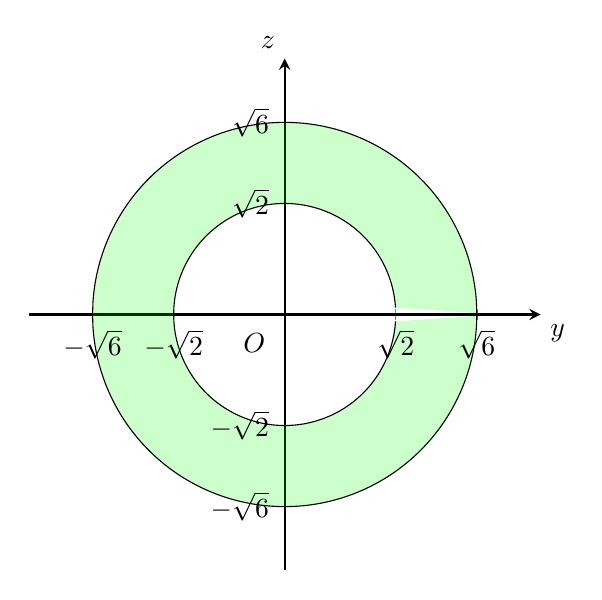
\begin{tikzpicture}
    \begin{axis}[standard,
            xtick={-2.44,-1.41,1.41,2.44},
            ytick={-2.44,-1.41,1.41,2.44},
            samples=1000,
            xlabel={$y$},
            ylabel={$z$},
          xmin=-2.5,xmax=2.5,           ymin=-2.5,ymax=2.5,
            x=1cm,
            y=1cm/1,        xticklabels={$-\sqrt{6}$,$-\sqrt{2}$, $\sqrt{2}$, $\sqrt{6}$},
            yticklabels={$-\sqrt{6}$,$-\sqrt{2}$, $\sqrt{2}$, $\sqrt{6}$}
           ]

    \node[anchor=center,label=south west:$O$] at (axis cs:0,0){};
\addplot[name path=F,domain={-2.44:2.44}]{sqrt(2.44^2-x^2)};
\addplot[name path=G,domain={-1.41:1.41}]{sqrt(1.41^2-x^2)};
\addplot[name path=H,domain={-2.44:2.44}]{-sqrt(2.44^2-x^2)};
\addplot[name path=I,domain={-1.41:1.41}]{-sqrt(1.41^2-x^2)};
\addplot[fill=green, fill opacity=0.2] fill between [of=F and G, soft clip={domain=-2.44:2.44}];
\addplot[fill=green, fill opacity=0.2] fill between [of=H and I, soft clip={domain=-2.44:2.44}];
    \end{axis}
    \end{tikzpicture}
}
\end{center}
With all these circles, it might be a good idea to switch to polar. Don't forget that since we're switching to polar, we need our Jacobian $r$.

The Jacobian is necessary because we are going from our original $x$,$y$,$z$ coordinates to $r$, $\theta$ coordiantes.

Based on the graph above,

Our lower and upper bounds for $r$ are $r=\sqrt{2}$ and $r=\sqrt{6}$, respectively.

Our lower and upper bounds for $\theta$ are $\theta =0$ and $\theta=2\pi$, respectively.

Let's evaluate the surface area integral.
\begin{align*}
    S&=\int_0^{2\pi}\int_{\sqrt{2}}^{\sqrt{6}}\lrp{\sqrt{4(r\cos\theta)^2+4(r\sin\theta)^2+1}}r\,dr\,d\theta\\
    &=\int_0^{2\pi}\int_{\sqrt{2}}^{\sqrt{6}}r\sqrt{4r^2\cos^2\theta+4r^2\sin^2\theta+1}\,dr\,d\theta\\
    &=\int_0^{2\pi}\int_{\sqrt{2}}^{\sqrt{6}}r\sqrt{4r^2\lrp{\cos^2\theta+\sin^2\theta}+1}\,dr\,d\theta\\
    &=\int_0^{2\pi}\int_{\sqrt{2}}^{\sqrt{6}}r\sqrt{4r^2+1}\,dr\,d\theta\tag{$\cos^2\theta+\sin^2\theta=1$}\\
    &=\int_0^{2\pi}\lrb{\frac{1}{12}(4r^2+1)^{3/2}}_{\sqrt{2}}^{\sqrt{6}}\,d\theta\tag{or do $u$-sub, $u=4r^2+1$}\\
    &=\int_0^{2\pi}\frac{1}{12}\lrp{4(6)+1}^{3/2}-\frac{1}{12}\lrp{4(2)+1}^{3/2}\,d\theta\\
    &=\int_0^{2\pi}\frac{49}{6}\,d\theta\tag{use a calculator}\\
    &=\lrb{\frac{49}{6}\theta}_0^{2\pi}\\
    &=\lrp{\frac{49}{6}}\lrp{2\pi}\\
    &=\boxed{\frac{49}{3}\pi}
\end{align*}
\phantomsection
\addcontentsline{toc}{subsection}{1(b)}\textbf{(b)} The region cut from the plane $x+2y+2z=5$ by $x=y^2$ and $x=2-y^2$

\Solution

Recall that if a surface is given by a function $g(x,y,z)=c$ that defines $z$ implicitly as a function of $x$ and $y$, then the area of surface is
\begin{equation*}
    S=\iint_R \frac{\norm{\nabla g}}{\left| g_z\right|}\,dA
\end{equation*}
Let $g(x,y,z)=x+2y+2z$. 

We'll have $z$ be the variable that is implicitly defined because our region is given in terms of $x$ and $y$.

Let's find $\displaystyle\frac{\norm{\nabla g}}{\left| g_z\right|} $.
\begin{align*}
    \nabla g&=\lra{1,2,2}\\
    g_z&=2\\
    \frac{\norm{\nabla g}}{\left|g_z\right|}&=\frac{\sqrt{1^2+2^2+2^2}}{\left|2\right|}=\frac{\sqrt{9}}{2}=\frac{3}{2}
\end{align*}

Let's find the region $R$ that we're integrating over.

The problem tells us that our region is between $x=y^2$ and $x=2-y^2$.

Graphically, our region looks like \begin{center}
\resizebox{3.5cm}{!}{
    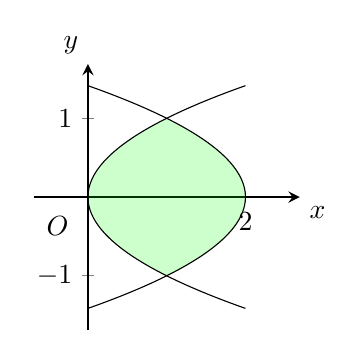
\begin{tikzpicture}
    \begin{axis}[standard,
            xtick={2},
            ytick={-1,1},
            samples=1000,
            xlabel={$x$},
            ylabel={$y$},
            xmin=-0.3,xmax=2.3,
            ymin=-1.3,ymax=1.3,
            x=1cm,
            y=1cm/1,
           ]
\node[anchor=center,label=south west:$O$] at (axis cs:0,0){};
\addplot[name path=F,domain={0:2}]{sqrt(2-x)};
\addplot[name path=G,domain={0:2}]{-sqrt(2-x)};
\addplot[fill=green, fill opacity=0.2] fill between [of=F and G, soft clip={domain=1:2}];
\addplot[name path=H,domain={0:2}]{sqrt(x)};
\addplot[name path=I,domain={0:2}]{-sqrt(x)};
\addplot[fill=green, fill opacity=0.2] fill between [of=H and I, soft clip={domain=0:1}];
    \end{axis}
    \end{tikzpicture}
}
\end{center}

Our lower and upper bounds for $x$ are $x=y^2$ and $x=2-y^2$, respectively.

Our lower and upper bounds for $y$ are $y=-1$ and $y=1$, respectively.

Let's evaluate the surface area integral.
\begin{align*}
    S&=\int_{-1}^1\int_{y^2}^{2-y^2}\frac{3}{2}\,dx\,dy\\
    &=\int_{-1}^1\lrb{\frac{3}{2}x}_{y^2}^{2-y^2}\,dy\\
    &=\int_{-1}^1\frac{3}{2}\lrp{2-y^2}-\frac{3}{2}y^2\,dy\\
    &=\int_{-1}^1 3-\frac{3}{2}y^2-\frac{3}{2}y^2\,dy\\
    &=\int_{-1}^1 3-3y^2\,dy\\
    &=\lrb{3y-y^3}_{-1}^1\\
    &=\big(3(1)-1^3\big)-\big(3(-1)-(-1)^3\big)\\
    &=\lrp{2}-\lrp{-2}\\
    &=\boxed{4}
\end{align*}

\phantomsection
\addcontentsline{toc}{subsection}{1(c)}\textbf{(c)} The region of $x^2-2y-2z=0$ above the triangle bounded by the lines $x=0$, $y=0$, and $y=3x$

\Solution

Recall that if a surface is given by a function $g(x,y,z)=c$ that defines $z$ implicitly as a function of $x$ and $y$, then the area of surface is
\begin{equation*}
    S=\iint_R \frac{\norm{\nabla g}}{\left| g_z\right|}\,dA
\end{equation*}
Let $g(x,y,z)=x^2-2y-2z$. 

We'll have $z$ be the variable that is implicitly defined because our region is given in terms of $x$ and $y$.

Let's find $\displaystyle\frac{\norm{\nabla g}}{\left| g_z\right|} $.
\begin{align*}
    \nabla g&=\lra{2x,-2,-2}\\
    g_z&=-2\\
    \frac{\norm{\nabla g}}{\left| g_z\right|}&=\frac{\sqrt{(2x)^2+(-2)^2+(-2)^2}}{\left|-2\right|}=\frac{\sqrt{4x^2+8}}{2}=\frac{\sqrt{4(x^2+2)}}{2}=\frac{\sqrt{4}\sqrt{x^2+2}}{2}=\sqrt{x^2+2}
\end{align*}
Let's find the region $R$ we're integrating over.

The problem tells us that we're bounded by the lines $x=0$, $y=0$, and $y=3x$.

Graphically, our region looks like \begin{center}
\resizebox{2.5cm}{!}{
    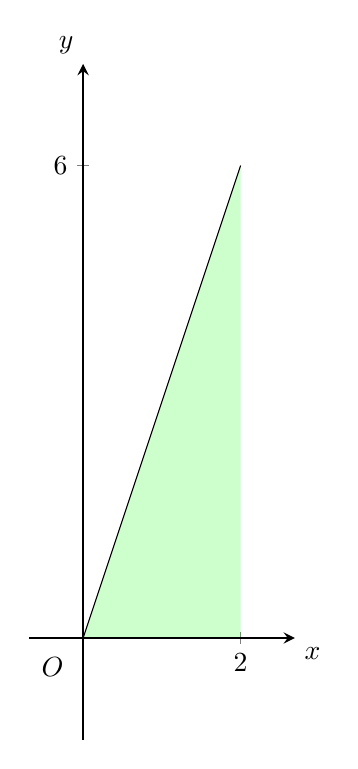
\begin{tikzpicture}
    \begin{axis}[standard,
            xtick={2},
            ytick={6},
            samples=1000,
            xlabel={$x$},
            ylabel={$y$},
            xmin=-0.3,xmax=2.3,
            ymin=-0.3,ymax=6.3,
            x=1cm,
            y=1cm/1,
           ]
\node[anchor=center,label=south west:$O$] at (axis cs:0,0){};
\addplot[name path=F,domain={0:2}]{3*x};
\addplot[name path=G,domain={0:2}]{0};
\addplot[fill=green, fill opacity=0.2] fill between [of=F and G, soft clip={domain=0:2}];
    \end{axis}
    \end{tikzpicture}
}
\end{center}

Our lower and upper bounds for $y$ are $y=0$ and $y=3x$, respectively.

Our lower and upper bounds for $x$ are $x=0$ and $x=2$, respectively.

Let's evaluate the surface area integral.
\begin{align*}
    \int_0^2\int_0^{3x}\sqrt{x^2+2}\,dy\,dx\\
    &=\int_0^2\lrb{y\sqrt{x^2+2}}_0^{3x}\,dx\\
    &=\int_0^2 3x\sqrt{x^2+2}\,dx\\
    &=\lrb{(x^2+2)^{3/2}}_0^2\tag{or do $u$-sub, $u=x^2+2$}\\
    &=\big(\lrp{2^2+2}^{3/2}\big)-\big(\lrp{0^2+2}^{3/2}\big)\\
    &=\lrp{6^{3/2}}-\lrp{2^{3/2}}\\
    &=\boxed{6\sqrt{6}-2\sqrt{2}}\tag{$a^{3/2}=\sqrt{a^3}=\sqrt{a^2(a)}=a\sqrt{a}$}
\end{align*}

\phantomsection
\addcontentsline{toc}{subsection}{1(d)}\textbf{(d)} The upper part of the cylinder $x^2+z^2=1$ between the planes $x=\pm\frac{1}{2}$ and $y=\pm\frac{1}{2}$.

\Solution

Recall that if a surface is given by a function $g(x,y,z)=c$ that defines $z$ implicitly as a function of $x$ and $y$, then the area of surface is
\begin{equation*}
    S=\iint_R \frac{\norm{\nabla g}}{\left| g_z\right|}\,dA
\end{equation*}
Let $g(x,y,z)=x^2+z^2$. 

We'll have $z$ be the variable that is implicitly defined because our region is given in terms of $x$ and $y$.

Let's find $\displaystyle\frac{\norm{\nabla g}}{\left| g_z\right|} $.
\begin{align*}
    \nabla g &=\lra{2x,0,2z}\\
    g_z&= 2z\\
    \frac{\norm{\nabla g}}{\left|g_z\right|}&=\frac{\sqrt{(2x)^2+0^2+(2z)^2}}{2z}\\
    &=\frac{\sqrt{4x^2+4z^2}}{2z}\\
    &=\frac{\sqrt{4(x^2+z^2)}}{2z}\\
    &=\frac{\sqrt{4(1)}}{2z}\tag{$x^2+z^2=1$}\\
    &=\frac{2}{2z}\\
    &=\frac{1}{z}\\
    &=\frac{1}{\sqrt{1-x^2}}\tag{$z^2=1-x^2\implies z=\sqrt{1-x^2}$}
\end{align*}
Let's find the region $R$ we're integrating over.

The problem tells us that we're bounded by the planes $x=\pm\frac{1}{2}$ and $y=\pm\frac{1}{2}$.

Graphically, our region looks like \begin{center}
\resizebox{3.5cm}{!}{
    \begin{tikzpicture}
    \begin{axis}[standard,
            xtick={-3,3},
            ytick={-3,3},
            samples=1000,
            xlabel={$x$},
            ylabel={$y$},
            xmin=-3.3,xmax=3.3,
            ymin=-3.3,ymax=3.3,
            x=1cm,
            y=1cm/1,
            xticklabels={$-\dfrac{1}{2}$, $\dfrac{1}{2}$},
            yticklabels={$-\dfrac{1}{2}$, $\dfrac{1}{2}$}
           ]
\node[anchor=center,label=south west:$O$] at (axis cs:0,0){};
\addplot[name path=F,domain={-3:3}]{3};
\addplot[name path=G,domain={-3:3}]{-3};
\addplot[fill=green, fill opacity=0.2] fill between [of=F and G, soft clip={domain=-3:3}];
    \end{axis}
    \end{tikzpicture}
}
\end{center}

Our lower and upper bounds for $y$ are $y=-\frac{1}{2}$ and $y=\frac{1}{2}$, respectively.

Our lower and upper bounds for $x$ are $x=-\frac{1}{2}$ and $x=\frac{1}{2}$, respectively.

Let's evaluate the surface area integral.
\begin{align*}
   S&= \int_{-1/2}^{1/2}\int_{-1/2}^{1/2}\frac{1}{\sqrt{1-x^2}}\,dx\,dy\\
    &=\int_{-1/2}^{1/2}\lrb{\sin^{-1}(x)}_{-1/2}^{1/2}\,dy\\
    &=\int_{-1/2}^{1/2}\sin^{-1}\lrp{\frac{1}{2}}-\sin^{-1}\lrp{-\frac{1}{2}}\,dy\\
    &=\int_{-1/2}^{1/2}\frac{\pi}{6}-\lrp{-\frac{\pi}{6}}\,dy\\
    &=\int_{-1/2}^{1/2}\frac{\pi}{3}\,dy\\
    &=\lrb{\frac{\pi}{3}y}_{-1/2}^{1/2}\\
    &=\Bigg(\frac{\pi}{3}\lrp{\frac{1}{2}}\Bigg)-\Bigg(\frac{\pi}{3}\lrp{-\frac{1}{2}}\Bigg)\\
    &=\lrp{\frac{\pi}{6}}-\lrp{-\frac{\pi}{6}}\\
    &=\frac{2\pi}{6}\\
    &=\boxed{\frac{\pi}{3}}
\end{align*}

\phantomsection
\addcontentsline{toc}{subsection}{1(e)}\textbf{(e)} The portion of the paraboloid $x=4-y^2-z^2$ above the region $1\leq y^2+z^2\leq 4$

\Solution

Recall that if a surface is given by a function $g(x,y,z)=c$ that defines $x$ implicitly as a function of $y$ and $z$, then the area of surface is
\begin{equation*}
    S=\iint_R \frac{\norm{\nabla g}}{\left| g_x\right|}\,dA
\end{equation*}
Let $g(x,y,z)=x+y^2+z^2$ ($x=4-y^2-z^2\implies x+y^2+z^2=4$). 

We'll have $x$ be the variable that is implicitly defined because our region is given in terms of $y$ and $z$ (and we get nice $yz$ circles from that).

Let's find $\displaystyle\frac{\norm{\nabla g}}{\left| g_x\right|} $.
\begin{align*}
    \nabla g &=\lra{1,2y,2z}\\
    g_x&=1\\
    \frac{\norm{\nabla g}}{\left|g_x\right|}&=\frac{\sqrt{1^2+(2y)^2+(2z)^2}}{1}=\sqrt{1+4y^2+4z^2}
\end{align*}
Let's find the region $R$ we're integrating over.

The problem tells us that $1\leq y^2+z^2\leq 4$. Our region is between two circles (one of radius $1$ and one of radius $2$).

Graphically, our region looks like  \begin{center}
\resizebox{4cm}{!}{
    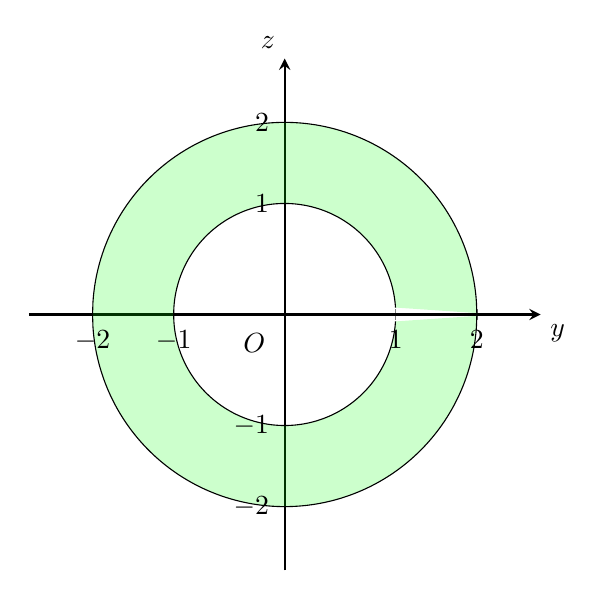
\begin{tikzpicture}
    \begin{axis}[standard,
            xtick={-2.44,-1.41,1.41,2.44},
            ytick={-2.44,-1.41,1.41,2.44},
            samples=1000,
            xlabel={$y$},
            ylabel={$z$},
          xmin=-2.5,xmax=2.5,           ymin=-2.5,ymax=2.5,
            x=1cm,
            y=1cm/1,        xticklabels={$-2$,$-1$, $1$, $2$},
            yticklabels={$-2$,$-1$, $1$, $2$}
           ]

    \node[anchor=center,label=south west:$O$] at (axis cs:0,0){};
\addplot[name path=F,domain={-2.44:2.44}]{sqrt(2.44^2-x^2)};
\addplot[name path=G,domain={-1.41:1.41}]{sqrt(1.41^2-x^2)};
\addplot[name path=H,domain={-2.44:2.44}]{-sqrt(2.44^2-x^2)};
\addplot[name path=I,domain={-1.41:1.41}]{-sqrt(1.41^2-x^2)};
\addplot[fill=green, fill opacity=0.2] fill between [of=F and G, soft clip={domain=-2.44:2.44}];
\addplot[fill=green, fill opacity=0.2] fill between [of=H and I, soft clip={domain=-2.44:2.44}];
    \end{axis}
    \end{tikzpicture}
}
\end{center}

With all these circles, it might be a good idea to switch to polar. Don't forget that since we're switching to polar, we need our Jacobian $r$.

The Jacobian is necessary because we are going from our original $x$,$y$,$z$ coordinates to $r$, $\theta$ coordinates.

Our lower and upper bounds for $r$ are $r=1$ and $r=2$, respectively.

Our lower and upper bounds for $\theta$ are $\theta=0$ and $\theta=2\pi$, respectively.

Let's evaluate the surface area integral.
\begin{align*}
    S&=\int_0^{2\pi}\int_1^2 \lrp{\sqrt{1+4\lrp{r\cos \theta}^2+4\lrp{r\sin \theta}^2}}r\,dr\,d\theta\\
    &=\int_0^{2\pi}\int_1^2 r\sqrt{1+4r^2\cos^2\theta+4r^2\sin^2\theta}\,dr\,d\theta\\
    &=\int_0^{2\pi}\int_1^2 r\sqrt{1+4r^2\lrp{\cos ^2 \theta+\sin ^2 \theta}}\,dr\,d\theta\\
    &=\int_0^{2\pi}\int_1^2 r\sqrt{1+4r^2}\,dr\,d\theta\tag{$\cos^2\theta+\sin^2\theta=1$}\\
    &=\int_0^{2\pi}\lrb{\frac{1}{12}(1+4r^2)^{3/2}}_1^2\,d\theta\tag{or do $u$-sub, $u=1+4r^2$}\\
    &=\int_0^{2\pi}\frac{1}{12}\big(1+4(2)^2\big)^{3/2}-\frac{1}{12}\big(1+4(1)^2\big)^{3/2}\,d\theta\\
    &=\int_0^{2\pi}\frac{1}{12}\lrp{17}^{3/2}-\frac{1}{12}(5)^{3/2}\,d\theta\\
    &=\lrb{\lrp{\frac{1}{12}(17)^{3/2}-\frac{1}{12}\lrp{5}^{3/2}}\theta}_0^{2\pi}\\
    &=\lrp{\frac{1}{12}(17)^{3/2}-\frac{1}{12}\lrp{5}^{3/2}}\lrp{2\pi}\\
    &=\lrp{\frac{1}{6}(17)^{3/2}-\frac{1}{6}(5)^{3/2}}\pi\\
    &={\lrp{\frac{17\sqrt{17}}{6}-\frac{5\sqrt{5}}{6}}\pi}\tag{$a^{3/2}=\sqrt{a^3}=\sqrt{a^2(a)}=a\sqrt{a}$}\\
    &=\boxed{\lrp{\frac{17\sqrt{17}-5\sqrt{5}}{6}}\pi}
\end{align*}
\phantomsection
\addcontentsline{toc}{subsection}{1(f)}\textbf{(f)} The surface $2x^{3/2}+2y^{3/2}-3z=0$ above the square $0\leq x\leq 1$, $0\leq y\leq 1$

\Solution

Recall that if a surface is given by a function $g(x,y,z)=c$ that defines $z$ implicitly as a function of $x$ and $y$, then the area of surface is
\begin{equation*}
    S=\iint_R \frac{\norm{\nabla g}}{\left| g_z\right|}\,dA
\end{equation*}
Let $g(x,y,z)=2x^{3/2}+2y^{3/2}-3z=0$. 

We'll have $z$ be the variable that is implicitly defined because our region is given in terms of $x$ and $y$.

Let's find $\displaystyle\frac{\norm{\nabla g}}{\left| g_z\right|} $.
\begin{align*}
    \nabla g&=\lra{3x^{1/2},3y^{1/2},-3}\\
    g_z&=-3\\
    \frac{\norm{\nabla g}}{\left|g_z\right|}&=\frac{\sqrt{\lrp{3x^{1/2}}^2+\lrp{3y^{1/2}}^2+(-3)^2}}{\left|-3\right|}=\frac{\sqrt{9x+9y+9}}{3}=\frac{\sqrt{9(x+y+1)}}{3}=\frac{3\sqrt{x+y+1}}{3}=\sqrt{x+y+1}
\end{align*}
Let's find the region $R$ we're integrating over.

The problem tells us that $0\leq x\leq 1$ and $0\leq y\leq 1$.

Graphically, our region looks like \begin{center}
\resizebox{3.5cm}{!}{
    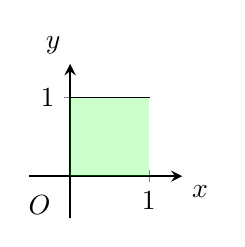
\begin{tikzpicture}
    \begin{axis}[standard,
            xtick={1},
            ytick={1},
            samples=1000,
            xlabel={$x$},
            ylabel={$y$},
            xmin=-0.3,xmax=1.2,
            ymin=-.3,ymax=1.2,
            x=1cm,
            y=1cm/1,
           ]
\node[anchor=center,label=south west:$O$] at (axis cs:0,0){};
\addplot[name path=F,domain={0:1}]{1};
\addplot[name path=G,domain={0:1}]{0};
\addplot[fill=green, fill opacity=0.2] fill between [of=F and G, soft clip={domain=0:1}];
    \end{axis}
    \end{tikzpicture}
}
\end{center}
Our lower and upper bounds for $y$ are $y=0$ and $y=1$, respectively.

Our lower and upper bounds for $x$ are $x=0$ and $x=1$, respectively.

Let's evaluate the surface area integral.
\begin{align*}
    S&=\int_0^1\int_0^1 \sqrt{x+y+1}\,dy\,dx\\
    &=\int_0^1 \lrb{\frac{2}{3}(x+y+1)^{3/2}}_0^1\,dx\tag{or do $u$-sub, $u=x+y+1$}\\
    &=\int_0^1 \lrp{\frac{2}{3}(x+1+1)^{3/2}}-\lrp{\frac{2}{3}(x+0+1)^{3/2}}\,dx\\
    &=\int_0^1 \frac{2}{3}\lrp{x+2}^{3/2}-\frac{2}{3}(x+1)^{3/2}\,dx\\
    &=\lrb{\frac{4}{15}(x+2)^{5/2}-\frac{4}{15}(x+1)^{5/2}}_0^1\tag{or do $u$-sub(s), $u_1=x+2$, $u_2=x+1$}\\
    &=\lrp{\frac{4}{15}(1+2)^{5/2}-\frac{4}{15}(1+1)^{5/2}}-\lrp{\frac{4}{15}(0+2)^{5/2}-\frac{4}{15}(0+1)^{5/2}}\\
    &=\lrp{\frac{4\lrp{3}^{5/2}}{15}-\frac{4(2)^{5/2}}{15}}-\lrp{\frac{4(2)^{5/2}}{15}-\frac{4}{15}}\\
    &={\frac{4\lrp{3}^{5/2}}{15}-\frac{4(2)^{5/2}}{15}}-{\frac{4(2)^{5/2}}{15}}+{\frac{4}{15}}\\
    &=\frac{4}{15}\lrp{3^{5/2}-2^{5/2}-2^{5/2}+1}\\
    &=\frac{4}{15}\lrp{3^23^{1/2}-2^22^{1/2}-2^22^{1/2}+1}\\
    &=\frac{4}{15}\lrp{9\sqrt{3}-4\sqrt{2}-4\sqrt{2}+1}\\
    &=\boxed{\frac{4}{15}\lrp{9\sqrt{3}-8\sqrt{2}+1}}
\end{align*}

\phantomsection
\addcontentsline{toc}{section}{Problem 2}\textbf{Problem 2} 

Find a formula for the area of a surface given by a function $y=f(x,z)$.

\Solution

If $y=f(x,z)$, then let's have our parameterization of the surface be
\begin{align*}
    \r(x,z)&=\lra{x,f(x,z),z}
\end{align*}
Recall that surface area can be represented as
\begin{align*}
    S&=\iint_R \norm{\frac{\partial \r}{\partial u}\times \frac{\partial \r}{\partial v}}\,dA
\end{align*}
Let's have $u=x$ and $v=z$.

Let's calculate the surface area given by a function $y=f(x,z)$.

If $\displaystyle   \r(x,z)=\lra{x,f(x,z),z}$, then
\begin{align*}
    \frac{\partial \r}{\partial x}&=\lra{1, \frac{\partial f}{\partial x}, 0}\\
    \frac{\partial \r}{\partial z}&=\lra{0, \frac{\partial f}{\partial z}, 1}\\
    \frac{\partial \r}{\partial x}\times \frac{\partial r}{\partial z} &= \lra{1, \frac{\partial f}{\partial x}, 0}\times \lra{0, \frac{\partial f}{\partial z}, 1}\\
    &=\begin{vmatrix}\i & \j & \k\\
    1 & \frac{\partial f}{\partial x} & 0\\
    0 & \frac{\partial f}{\partial z} & 1\end{vmatrix}\\
    &=\lrp{\frac{\partial f}{\partial x}-0}\i-\lrp{1-0}\j+\lrp{\frac{\partial f}{\partial z}-0}\k\\
    &=\lra{\frac{\partial f}{\partial x},1,\frac{\partial f}{\partial z}}\\
    \norm{\frac{\partial \r}{\partial x}\times \frac{\partial r}{\partial z}}&=\sqrt{\lrp{\frac{\partial f}{\partial x}}^2+1^2+\lrp{\frac{\partial f}{\partial z}}^2}\\
    &=\sqrt{1+\lrp{\frac{\partial f}{\partial x}}^2+\lrp{\frac{\partial f}{\partial z}}^2}
\end{align*}
Therefore, the formula for the area of a surface  given by a function $y=f(x,z)$ is
\begin{equation*}
   \boxed{ S=\iint_R \sqrt{1+\lrp{\frac{\partial f}{\partial x}}^2+\lrp{\frac{\partial f}{\partial z}}^2}\,dA}
\end{equation*}
\newpage
\phantomsection
\addcontentsline{toc}{section}{Problem 3}\textbf{Problem 3} 

Find a parametrization for the surface obtained by revolving a smooth curve given
by $y = f(x) \geq0$, $a \geq x \geq b$, around the $x$-axis and show that the surface area is
\begin{equation*}
    S=\int_a^b 2\pi f(x)\sqrt{1+f'(x)^2}\,dx
\end{equation*}
(\textit{Hint}: Use cylindrical coordinates $x$ and $\theta$.)

\Solution

Let's draw the surface to get a good idea of what we're looking at.

\tikzset{every picture/.style={line width=0.75pt}} %set default line width to 0.75pt        
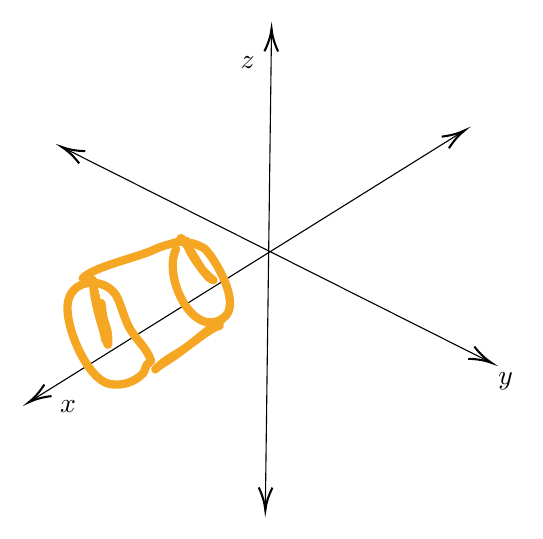
\begin{tikzpicture}[x=0.75pt,y=0.75pt,yscale=-1,xscale=1]
%uncomment if require: \path (0,300); %set diagram left start at 0, and has height of 300

%Straight Lines [id:da382120260672669] 
\draw    (193.19,263.33) -- (196.14,35.33) ;
\draw [shift={(196.17,33.33)}, rotate = 90.74] [color={rgb, 255:red, 0; green, 0; blue, 0 }  ][line width=0.75]    (10.93,-3.29) .. controls (6.95,-1.4) and (3.31,-0.3) .. (0,0) .. controls (3.31,0.3) and (6.95,1.4) .. (10.93,3.29)   ;
\draw [shift={(193.17,265.33)}, rotate = 270.74] [color={rgb, 255:red, 0; green, 0; blue, 0 }  ][line width=0.75]    (10.93,-3.29) .. controls (6.95,-1.4) and (3.31,-0.3) .. (0,0) .. controls (3.31,0.3) and (6.95,1.4) .. (10.93,3.29)   ;
%Straight Lines [id:da6800922508330479] 
\draw    (287.47,83.39) -- (80.86,212.27) ;
\draw [shift={(79.17,213.33)}, rotate = 328.04] [color={rgb, 255:red, 0; green, 0; blue, 0 }  ][line width=0.75]    (10.93,-3.29) .. controls (6.95,-1.4) and (3.31,-0.3) .. (0,0) .. controls (3.31,0.3) and (6.95,1.4) .. (10.93,3.29)   ;
\draw [shift={(289.17,82.33)}, rotate = 148.04] [color={rgb, 255:red, 0; green, 0; blue, 0 }  ][line width=0.75]    (10.93,-3.29) .. controls (6.95,-1.4) and (3.31,-0.3) .. (0,0) .. controls (3.31,0.3) and (6.95,1.4) .. (10.93,3.29)   ;
%Straight Lines [id:da3850032882218606] 
\draw    (96.95,91.23) -- (300.38,193.44) ;
\draw [shift={(302.17,194.33)}, rotate = 206.68] [color={rgb, 255:red, 0; green, 0; blue, 0 }  ][line width=0.75]    (10.93,-3.29) .. controls (6.95,-1.4) and (3.31,-0.3) .. (0,0) .. controls (3.31,0.3) and (6.95,1.4) .. (10.93,3.29)   ;
\draw [shift={(95.17,90.33)}, rotate = 26.68] [color={rgb, 255:red, 0; green, 0; blue, 0 }  ][line width=0.75]    (10.93,-3.29) .. controls (6.95,-1.4) and (3.31,-0.3) .. (0,0) .. controls (3.31,0.3) and (6.95,1.4) .. (10.93,3.29)   ;
%Shape: Free Drawing [id:dp18739730235356022] 
\draw  [color={rgb, 255:red, 245; green, 166; blue, 35 }  ,draw opacity=1 ][line width=3] [line join = round][line cap = round] (114.17,165.5) .. controls (114.5,167.83) and (114.67,170.2) .. (115.17,172.5) .. controls (115.68,174.87) and (116.77,177.11) .. (117.17,179.5) .. controls (117.5,181.47) and (117.76,187.41) .. (117.17,185.5) .. controls (114.55,177.13) and (110.17,163.78) .. (110.17,154.5) .. controls (110.17,153.83) and (110.03,155.85) .. (110.17,156.5) .. controls (112.03,165.53) and (114.17,174.5) .. (116.17,183.5) ;
%Shape: Free Drawing [id:dp5667850848241781] 
\draw  [color={rgb, 255:red, 245; green, 166; blue, 35 }  ,draw opacity=1 ][line width=3] [line join = round][line cap = round] (138.17,193.5) .. controls (135.8,186.4) and (130.39,182.95) .. (127.17,176.5) .. controls (125.33,172.82) and (123.93,167.61) .. (122.17,163.5) .. controls (117.75,153.19) and (100.78,152.72) .. (98.17,164.5) .. controls (95.73,175.46) and (107.39,202.54) .. (118.17,204.5) .. controls (124.95,205.73) and (130.53,203.13) .. (134.17,199.5) .. controls (135.53,198.14) and (135.32,194.5) .. (137.17,194.5) ;
%Shape: Free Drawing [id:dp4437707713647747] 
\draw  [color={rgb, 255:red, 245; green, 166; blue, 35 }  ,draw opacity=1 ][line width=3] [line join = round][line cap = round] (105.17,153.5) .. controls (110.91,147.75) and (132.21,143.48) .. (140.17,139.5) .. controls (142.7,138.23) and (146.57,137.36) .. (149.17,136.5) .. controls (150.01,136.22) and (156.64,135.5) .. (154.17,135.5) ;
%Shape: Free Drawing [id:dp7952514199468889] 
\draw  [color={rgb, 255:red, 245; green, 166; blue, 35 }  ,draw opacity=1 ][line width=3] [line join = round][line cap = round] (155.17,135.5) .. controls (155.17,140.15) and (163.79,151.12) .. (166.17,153.5) .. controls (166.27,153.6) and (168.17,154.5) .. (168.17,154.5) .. controls (168.17,154.5) and (163.65,150.91) .. (162.17,148.5) .. controls (161.54,147.48) and (152.17,131.59) .. (152.17,134.5) ;
%Shape: Free Drawing [id:dp678572410386636] 
\draw  [color={rgb, 255:red, 245; green, 166; blue, 35 }  ,draw opacity=1 ][line width=3] [line join = round][line cap = round] (150.17,139.5) .. controls (143.55,152.74) and (158.45,183.54) .. (173.17,172.5) .. controls (181.94,165.92) and (169,144.33) .. (164.17,139.5) .. controls (163.36,138.7) and (155.17,134.66) .. (155.17,137.5) ;
%Shape: Free Drawing [id:dp24234829473554076] 
\draw  [color={rgb, 255:red, 245; green, 166; blue, 35 }  ,draw opacity=1 ][line width=3] [line join = round][line cap = round] (171.17,174.5) .. controls (171.5,174.17) and (171.83,173.83) .. (172.17,173.5) ;
%Shape: Free Drawing [id:dp2574885815305624] 
\draw  [color={rgb, 255:red, 245; green, 166; blue, 35 }  ,draw opacity=1 ][line width=3] [line join = round][line cap = round] (168.17,176.5) .. controls (162.6,180.67) and (160.65,182.78) .. (154.17,187.5) .. controls (151.62,189.35) and (148.78,190.76) .. (146.17,192.5) .. controls (144,193.94) and (142.01,195.66) .. (140.17,197.5) .. controls (139.83,197.83) and (140.79,196.79) .. (141.17,196.5) .. controls (144.01,194.29) and (147.25,192.62) .. (150.17,190.5) .. controls (156.36,186) and (168.18,176.5) .. (171.17,176.5) ;

% Text Node
\draw (180,45.4) node [anchor=north west][inner sep=0.75pt]    {$z$};
% Text Node
\draw (93,211.4) node [anchor=north west][inner sep=0.75pt]    {$x$};
% Text Node
\draw (304.17,197.73) node [anchor=north west][inner sep=0.75pt]    {$y$};


\end{tikzpicture}

Our top view of the surface looks like
\begin{center}
\resizebox{5cm}{!}{
    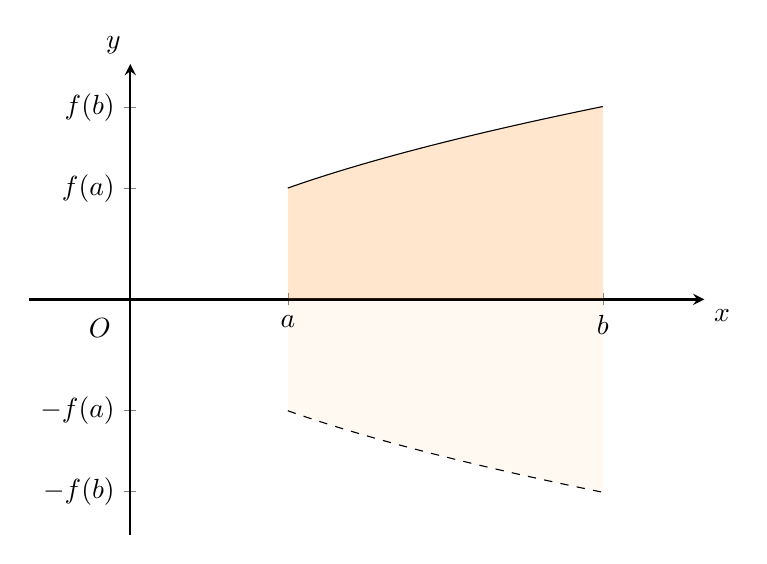
\begin{tikzpicture}
    \begin{axis}[standard,
            xtick={2,6},
            ytick={-2.44,-1.41, 1.41, 2.44},
            samples=1000,
            xlabel={$x$},
            ylabel={$y$},
            xmin=-0.3,xmax=6.3,
            ymin=-2.3,ymax=2.3,
            x=1cm,
            y=1cm/1,
            xticklabels={$a$, $b$},
            yticklabels={$-f(b)$, $-f(a)$, $f(a)$, $f(b)$}
           ]
\node[anchor=center,label=south west:$O$] at (axis cs:0,0){};
\addplot[name path=F,domain={2:6}]{sqrt(x)};
\addplot[name path=G,domain={2:6}]{0};
\addplot[fill=orange, fill opacity=0.2] fill between [of=F and G, soft clip={domain=2:6}];
\addplot[dashed,name path=H,domain={2:6}]{-sqrt(x)};
\addplot[fill=orange, fill opacity=0.05] fill between [of=H and G, soft clip={domain=2:6}];
    \end{axis}
    \end{tikzpicture}
}
\end{center}
Our front view of the surface looks like \begin{center}
\resizebox{5cm}{!}{
    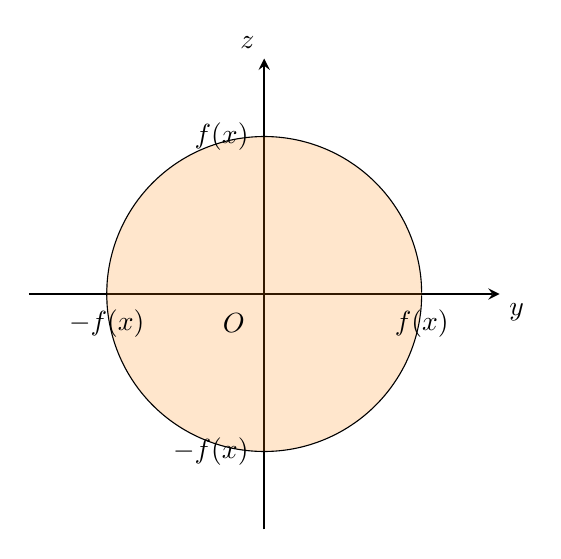
\begin{tikzpicture}
    \begin{axis}[standard,
            xtick={-2,2},
            ytick={-2,2},
            samples=1000,
            xlabel={$y$},
            ylabel={$z$},
          xmin=-2.3,xmax=2.3,           ymin=-2.3,ymax=2.3,
            x=1cm,
            y=1cm/1,        xticklabels={$-f(x)$, $f(x)$},
            yticklabels={$-f(x)$, $f(x)$}
           ]

    \node[anchor=center,label=south west:$O$] at (axis cs:0,0){};
\addplot[name path=F,domain={-2:2}]{sqrt(4-x^2)};
\addplot[name path=G,domain={-2:2}]{-sqrt(4-x^2)};
\addplot[fill=orange, fill opacity=0.2] fill between [of=F and G, soft clip={domain=-2:2}];
    \end{axis}
    \end{tikzpicture}
}
\end{center}
From the front view, we can see that we have a circle of radius $r$ where $r=y=f(x)$ and $\theta$ is the angle between the $xy$-plane and $z$. Just like how we do polar in $xy$, let $z=r\sin \theta = f(x)\sin \theta$, and $y=r\cos\theta =f(x)\cos \theta$.

Therefore, let's have our parameterization for the surface be
\begin{align*}
    \r(x,\theta)&=\lra{x, f(x)\cos\theta, f(x)\sin \theta}
\end{align*}
Our lower and upper bounds for $x$ will be $x=a$ and $x=b$, respectively (given in the problem).

Based on the front view and the problem, we're going around the entire $x$-axis. Therefore, our lower and upper bounds for $\theta$ will be $\theta =0$ and $\theta=2\pi$, respectively.

Recall that surface area can be represented as
\begin{align*}
    S&=\iint_R \norm{\frac{\partial \r}{\partial u}\times \frac{\partial \r}{\partial v}}\,dA
\end{align*}
Let's have $u=x$ and $v=\theta$.

Let's calculate the surface area given by a function $y=f(x,z)$.

If $\displaystyle   \r(x,z)=\lra{x,f(x)\cos\theta, f(x)\sin\theta}$, then 
\begin{align*}
    \frac{\partial \r}{\partial x}&=\lra{1, f'(x)\cos\theta, f'(x)\sin\theta}\\
    \frac{\partial \r}{\partial \theta}&=\lra{0,-f(x)\sin\theta, f(x)\cos\theta}\\
     \frac{\partial \r}{\partial x}\times \frac{\partial \r}{\partial \theta}&=\lra{1, f'(x)\cos\theta, f'(x)\sin\theta}\times \lra{0,-f(x)\sin\theta, f(x)\cos\theta}\\
     &=\begin{vmatrix}
     \i &\j & \k\\
     1 & f'(x)\cos\theta & f'(x)\sin\theta\\
     0 & -f(x)\sin\theta & f(x)\cos\theta
     \end{vmatrix}\\
     &=\lrp{f(x)f'(x)\cos^2\theta+f(x)f'(x)\sin^2\theta}\i-\lrp{f(x)\cos\theta-0}\j+\lrp{-f(x)\sin\theta-0}\k\\
     &=\big(f(x)f'(x)\lrp{\cos^2\theta+\sin^2\theta}\big)\i-\lrp{f(x)\cos\theta}\j+\lrp{-f(x)\sin\theta}\k\\
     &=\lrp{f(x)f'(x)}\i-\lrp{f(x)\cos\theta}\j+\lrp{-f(x)\sin\theta}\k\tag{$\cos^2\theta+\sin^2\theta=1$}\\
     &=\lra{f(x)f'(x),-f(x)\cos\theta, -f(x)\sin\theta}\\
     \norm{ \frac{\partial \r}{\partial x}\times \frac{\partial \r}{\partial \theta}}&=\sqrt{f(x)^2f'(x)^2+f(x)^2\cos^2\theta+f(x)^2\sin^2\theta}\\
     &=\sqrt{f(x)^2f'(x)^2+f(x)^2\lrp{\cos^2\theta+\sin^2\theta}}\\
     &=\sqrt{f(x)^2f'(x)^2+f(x)^2}\tag{$\cos^2\theta+\sin^2\theta=1$}\\
     &=\sqrt{f(x)^2\big(f'(x)^2+1\big)}\\
     &=f(x)\sqrt{f'(x)^2+1}\tag{$y=f(x)\geq 0$}\\
     &=f(x)\sqrt{1+f'(x)^2}
\end{align*}
Let's evaluate our surface area integral.
\begin{align*}
    S&=\int_a^b\int_0^{2\pi} f(x)\sqrt{1+f'(x)^2}\,d\theta\,dx\\
    &=\int_a^b \lrb{\theta f(x)\sqrt{1+f'(x)^2}}_0^{2\pi}\,dx\\
    &=\int_a^b 2\pi f(x)\sqrt{1+f'(x)^2}\,dx
\end{align*}

\qed
\end{document}
